\documentclass[a4paper]{article}
\usepackage[T1]{fontenc}
\usepackage[utf8]{inputenc}
\usepackage{geometry}
\usepackage{fancyhdr}
% \usepackage[italian]{babel}
\usepackage{amsmath,amssymb,amsfonts,amsthm}

\usepackage{hyperref}	% enable hyperlinks to referenced elements
\hypersetup{
	colorlinks=true,
	linkcolor=cyan,
	citecolor=cyan,
	linkcolor=cyan
}

\usepackage{subcaption} % per poter usare subfigure devi importare questo package
\usepackage{graphicx} % per usare includegraphics
\usepackage{float} % per avere H
\graphicspath{{./immagini/}}    


% \newcommand{\rfig}[1]{Figure~\ref{fig:#1}}
\newcommand{\rfig}[1]{Figure~\ref{#1}}

\begin{document}

\begin{center}
    {\Large Computer Vision - Lab 6}

    \vspace*{0.25cm}

    {\Large Keypoints, Descriptors and Matching}

    \vspace*{0.35cm}

    {\large Your Name - Your ID}
\end{center}

\section{Object detection}

The goal of the lab was to find the instances of an object in a scene using the keypoint descriptors.
To find the object in a scene, first we processed the images to extract the features using the \emph{SIFT} method (Section~\ref{sss:sift}), then matched the descriptors using a \emph{brute-force} matcher and computed the homography using \emph{RANSAC} algorithm (Section~\ref{sss:matching}).
After some hand tuning of the parameters, the object can generally be found, but a single set of parameters does not work well on all scenes (Section~\ref{sss:results}).

\subsection{SIFT keypoints and descriptors}
\label{sss:sift}
The key idea behind SIFT is that corners might not appear as corner when the image is scaled. For example the \emph{Harris} corner detector is robust with respect to rotation, but is highly dependent to the window size that is used: if a window is too small to cover the entire corner, it might look like a line and not be detected.
The \emph{Scale-Invariant} Feature Transform solves exactly this problem, by detecting features using \emph{scale-space} filtering.
The local extrema are found by comparing each pixel with its 8 neighbours as well as the 9 pixels in the previous and next scale, computed using the Difference of Gaussians.
After computing the potential keypoint locations, the ones that have intensity lower than a certain threshold are rejected.
Edges are also detected in this way, and are filtered using the Hessian matrix, comparing the ratio of the eigenvalues with a second threshold. Then, an orientation is associated to each keypoint, to make the method robust to rotation. Finally, a descriptor is generated from the keypoint.

The SIFT method is implemented in the \texttt{cv::xfeatures2d::SIFT} library, descriptors can be extracted with \texttt{detectAndCompute()}.

Descriptors in two different images are then matched, as explained in the next section.

\subsection{Descriptor matching}
\label{sss:matching}
The brute-force matcher simply picks each descriptor of the first image and matches it to all descriptors in the second, returning the closest one according to some similarity metric between the descriptors (\rfig{fig:allmatches}).
% A \emph{FLANN} based matcher performs faster on larger datasets, but was not needed in this case.
The matches were filtered by finding the minimum distance between two keypoints, and keeping only the matches with distance less than \emph{ratio*minDist} (\rfig{fig:goodmatches}).
Then the homography matrix is computed, using the RANSAC method to establish whether a pair of point is an inlier, further reducing the number of matches considered good (\rfig{fig:ransacmatches}).
A box as big as the original image is then translated on the scene to show the location of the object found (\rfig{fig:foundobject}).

The brute force matcher is implemented in \texttt{cv::BFMatcher}, and the matches are computed using \texttt{match()}. The RANSAC algorithm is implemented by \texttt{cv::findHomography()}, and the bounding box is projected using \texttt{cv::perspectiveTransform()}.

% \begin{figure}[H]
\begin{figure}[h!]
    \centering
    \begin{subfigure}[b]{0.45\textwidth}
        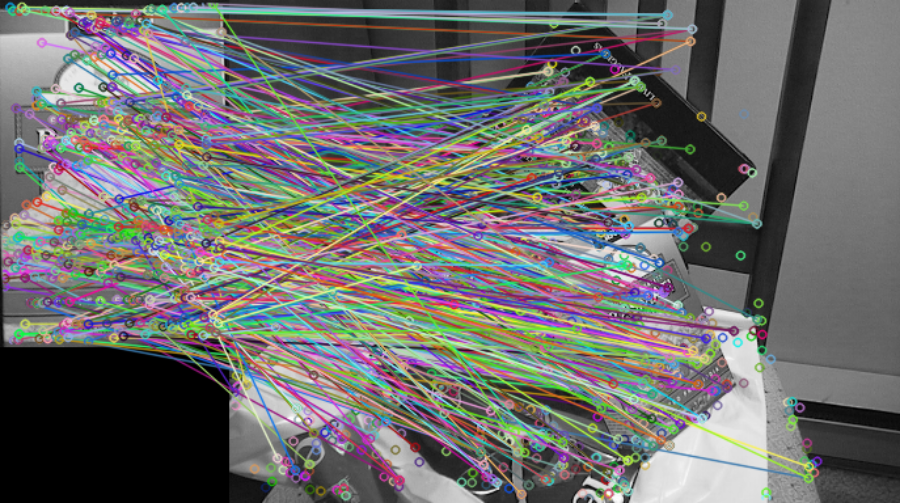
\includegraphics[width=\textwidth]{Data2_AllMatches_0_0_ratio3_RRT3_NF1000.png}
        \caption{All matches}
        \label{fig:allmatches}
    \end{subfigure}
    \quad
    \begin{subfigure}[b]{0.45\textwidth}
        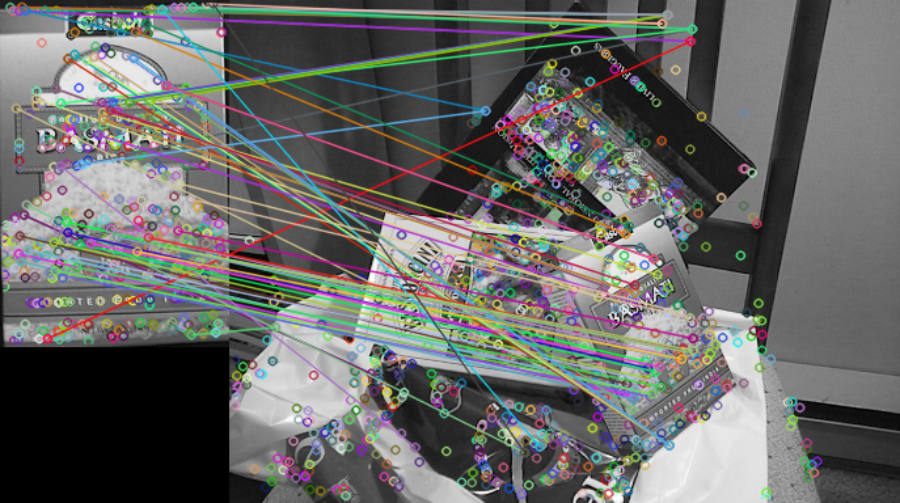
\includegraphics[width=\textwidth]{Data2_GoodMatches_0_0_ratio3_RRT3_NF1000.png}
        \caption{Good matches}
        \label{fig:goodmatches}
    \end{subfigure}
    \\
    \begin{subfigure}[b]{0.45\textwidth}
        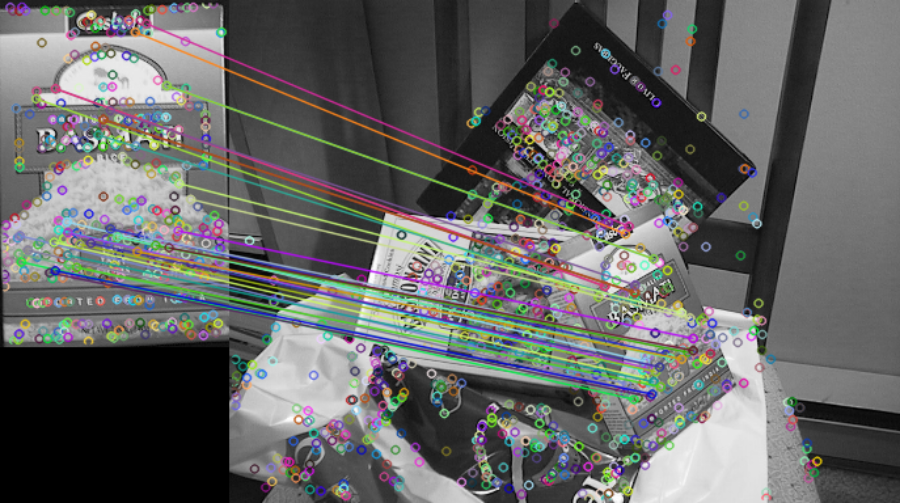
\includegraphics[width=\textwidth]{Data2_RANMatches_0_0_ratio3_RRT3_NF1000.png}
        \caption{RANSAC inliers}
        \label{fig:ransacmatches}
    \end{subfigure}
    \quad
    \begin{subfigure}[b]{0.45\textwidth}
        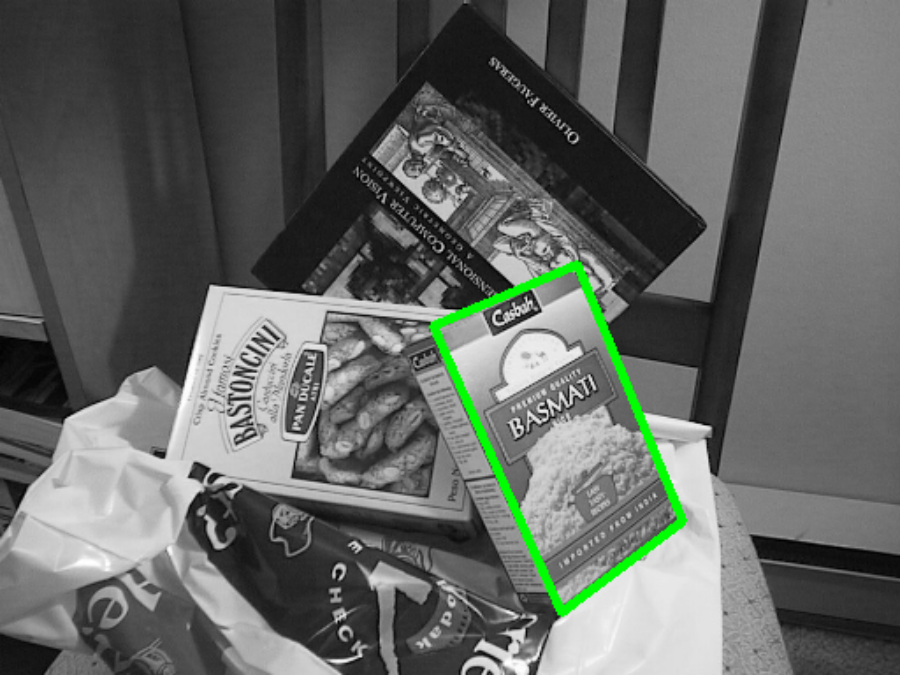
\includegraphics[width=\textwidth]{Data2_FoundMatches_0_0_ratio3_RRT3_NF1000.png}
        \caption{Detected object}
        \label{fig:foundobject}
    \end{subfigure}
    \caption{Matching and object detection example (dataset 2, object 1, scene 1)}
    \label{fig:matches}
\end{figure}

\subsection{Results}
\label{sss:results}
All the values used to extract the SIFT descriptor are the default one, as lowering the thresholds can provide more keypoints, but of lower quality, except for the \texttt{nFeatures} parameter, that was set to $500$, $1000$ and $2000$. The \texttt{ratio}s tested were $3$ and $9$, and the \texttt{ransacReprojectionThreshold (RRT)} was set to $3$ and $9$ as well.

Generally speaking, more features lead to better results (\rfig{fig:data1better}); in only one case the box was worse when using 1000 features instead of 500 (\rfig{fig:data4worse}).

When a lot of descriptors are found by SIFT, a ratio of 3 and RRT of 3 work well, as happens in the first three datasets. For the last one, less than 500 features are found for some of the object images, so a higher ratio and RRT can lead to better results: the individual matches used might be of worse quality, but overall they are more evenly spread around the object image, allowing a better result.
For example in \rfig{fig:data430331}, the matches are the best ones, but are concentrated in the center of the image, and the box cannot be computed well.
With higher values of ratio or ransacReprojectionThreshold, more matches are used to compute the homography matrix, and the results improve.
Out of 173 possible matches, 134 are kept with ratio 3, while 173 are used with ratio 9; of those matches, the RANSAC inliers are:
\begin{equation*}
    \begin{array}[h]{ccc}
         & \text{ratio 3} & \text{ratio 9} \\
        \text{RRT 3} & 20 & 17 \\
        \text{RRT 9} & 28 & 30 \\
    \end{array}
\end{equation*}

\begin{figure}[h!]
    \begin{subfigure}[b]{0.45\textwidth}
        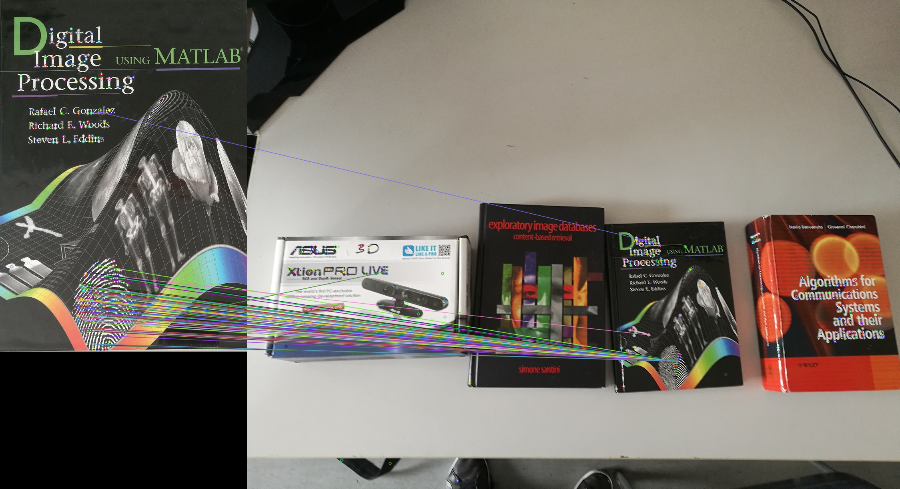
\includegraphics[width=\textwidth]{Data1_DetRANMatches_0_0_ratio3_RRT3_NF500.png}
        \caption{500 features}
        \label{fig:data100335}
    \end{subfigure}
    \quad
    \begin{subfigure}[b]{0.45\textwidth}
        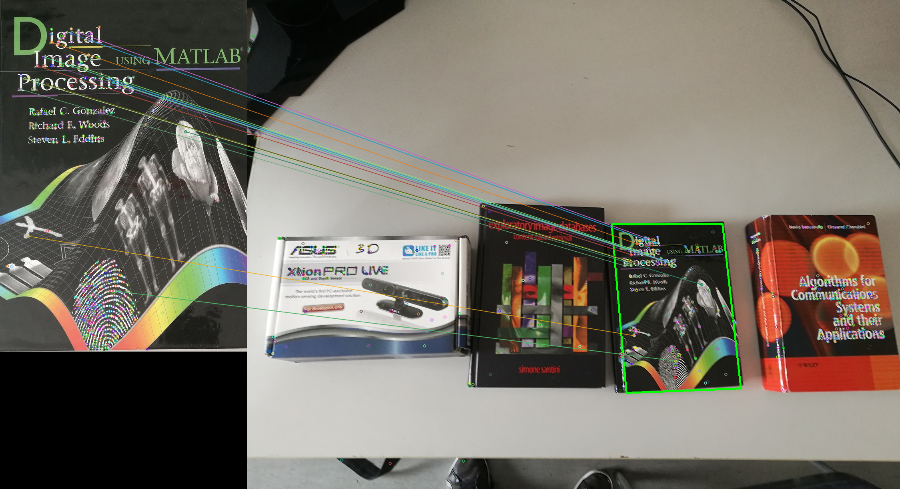
\includegraphics[width=\textwidth]{Data1_DetRANMatches_0_0_ratio3_RRT3_NF1000.png}
        \caption{1000 features}
        \label{fig:data100331}
    \end{subfigure}
    \caption{Better results with more features (dataset 1, object 1, scene 1, ratio 3, RRT 3)}
    \label{fig:data1better}
\end{figure}

\begin{figure}[h!]
    \begin{subfigure}[b]{0.45\textwidth}
        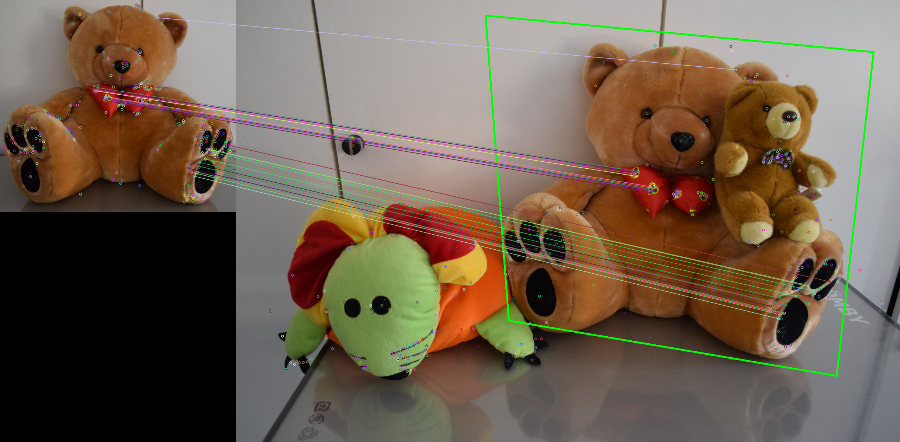
\includegraphics[width=\textwidth]{Data4_DetRANMatches_0_0_ratio9_RRT3_NF500.png}
        \caption{500 features}
        \label{fig:data400935}
    \end{subfigure}
    \quad
    \begin{subfigure}[b]{0.45\textwidth}
        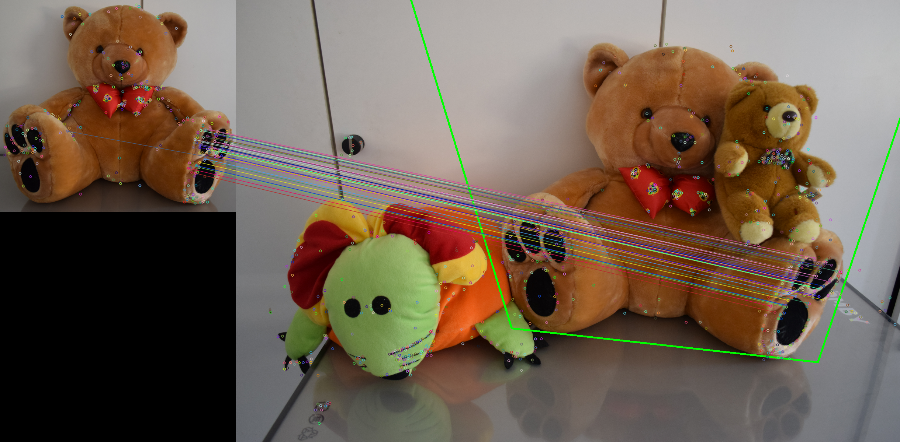
\includegraphics[width=\textwidth]{Data4_DetRANMatches_0_0_ratio9_RRT3_NF1000.png}
        \caption{1000 features}
        \label{fig:data400931}
    \end{subfigure}
    \caption{Worse results with more features (dataset 4, object 1, scene 1, ratio 9, RRT 3)}
    \label{fig:data4worse}
\end{figure}

\begin{figure}[h!]
    \begin{subfigure}[b]{0.45\textwidth}
        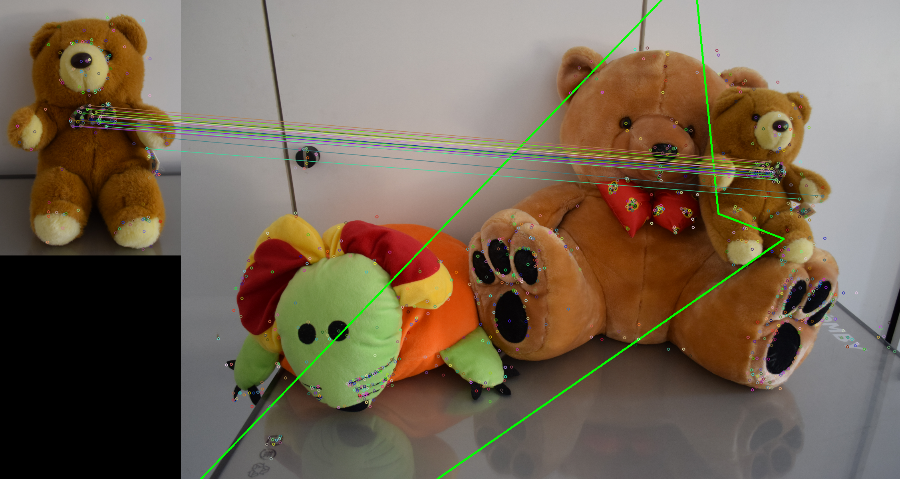
\includegraphics[width=\textwidth]{Data4_DetRANMatches_3_0_ratio3_RRT3_NF1000.png}
        \caption{Ratio 3, RRT 3}
        \label{fig:data430331}
    \end{subfigure}
    \quad
    \begin{subfigure}[b]{0.45\textwidth}
        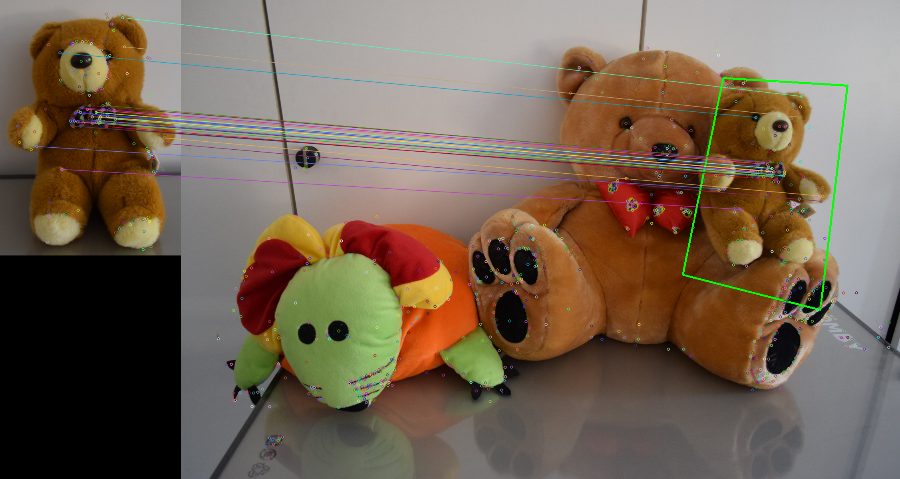
\includegraphics[width=\textwidth]{Data4_DetRANMatches_3_0_ratio3_RRT9_NF1000.png}
        \caption{Ratio 3, RRT 9}
        \label{fig:data430391}
    \end{subfigure}
    \\
    \begin{subfigure}[b]{0.45\textwidth}
        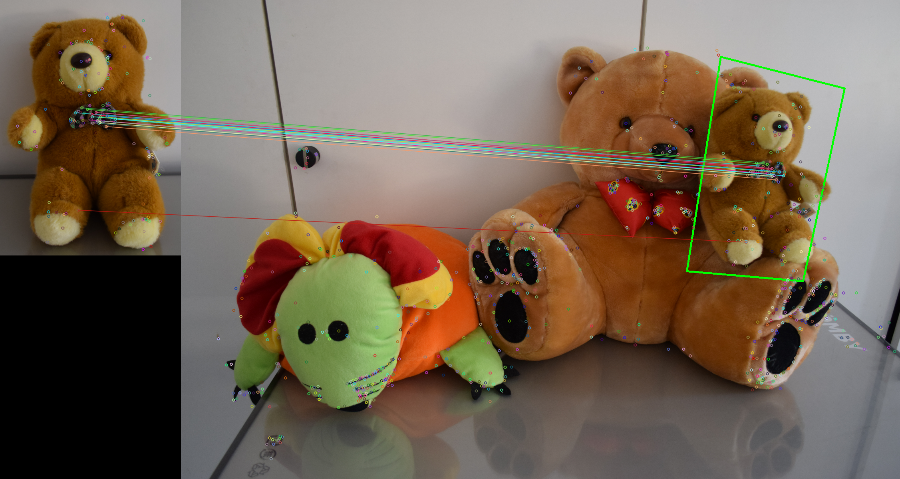
\includegraphics[width=\textwidth]{Data4_DetRANMatches_3_0_ratio9_RRT3_NF1000.png}
        \caption{Ratio 9, RRT 3}
        \label{fig:data430931}
    \end{subfigure}
    \quad
    \begin{subfigure}[b]{0.45\textwidth}
        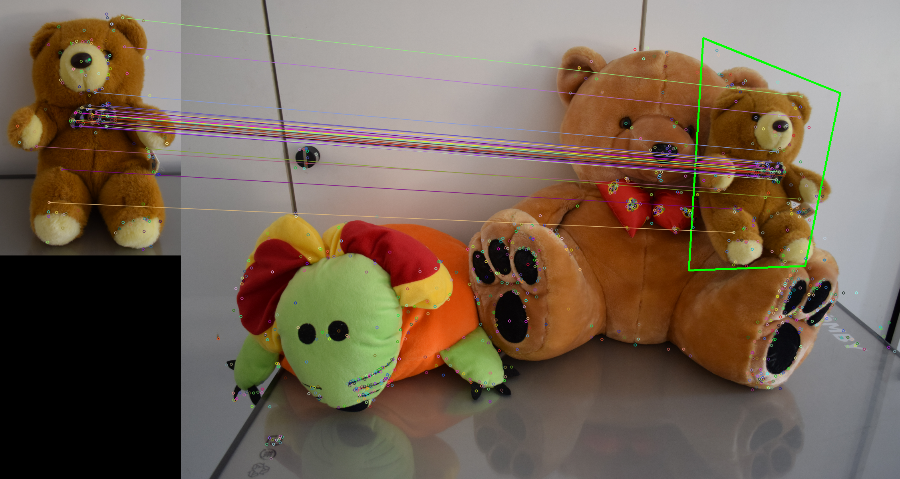
\includegraphics[width=\textwidth]{Data4_DetRANMatches_3_0_ratio9_RRT9_NF1000.png}
        \caption{Ratio 9, RRT 9}
        \label{fig:data430991}
    \end{subfigure}
    \caption{Better results with higher ratio and RRT (dataset 4, object 4, scene 1)}
    \label{fig:data4rr}
\end{figure}

\end{document}
